\documentclass[xcolor=dvipsnames]{beamer}

% Copyright 2010 by Brendan W. McAdams <brendan@10gen.com>
%
% You may redistribute the content of this presentation for your own needs 
% provided you give credit to its author. In other words: "Don't be a dick."
% % Latex code based upon the "Generic Presentation 15-45 minutes" template from Beamer.


\mode<presentation>
{
  % \usetheme{Dresden}      
  \usetheme{Madrid}
  \setbeamercolor{structure}{fg=OliveGreen!125!black} 
        
  % \usecolortheme{dolphin}
  \setbeamercovered{transparent}
}


\usepackage{hyperref}
\usepackage{xcolor}
\usepackage{listings}

\hypersetup{backref,  
pdfpagemode=FullScreen,  
colorlinks=false}

 % "define" Scala
\lstdefinelanguage{Scala}{
   morekeywords={abstract,case,catch,class,def,%
     do,else,extends,false,final,finally,%
     for,forSome,if,implicit,import,lazy,%
     match,mixin,%
     new,null,object,override,package,%
     private,protected,requires,return,sealed,%
     super,this,throw,trait,true,try,%
     type,val,var,while,with,yield},
   otherkeywords={=>,<-,<\%,<:,>:,\#,@},
   sensitive=true,
   morecomment=[l]{//},
   morecomment=[n]{/*}{*/},
   morestring=[b]",
   morestring=[b]',
   morestring=[b]"""
 }


\lstdefinelanguage{JavaScript}{
    keywords={typeof, new, true, false, catch, function, return, null, catch, switch, var, if, in, while, do, else, case, break}
    keywordstyle=\color{blue}\bfseries,
    ndkeywords={class, export, boolean, throw, implements, import, this},
    ndkeywordstyle=\color{darkgray}\bfseries,
    identifierstyle=\color{black},
    sensitive=false,
    comment=[l]{//},
    morecomment=[s]{/*}{*/},
    commentstyle=\color{purple}\ttfamily,
    stringstyle=\color{red}\ttfamily,
    morestring=[b]',
    morestring=[b]"
}
\usepackage{caption}
\DeclareCaptionFont{white}{\color{white}}
\DeclareCaptionFormat{listing}{\colorbox{black}{\parbox{\textwidth}{#1#2#3}}}
\captionsetup[lstlisting]{format=listing,labelfont=white,textfont=white}


\usepackage{color}
\definecolor{dkgreen}{rgb}{0,0.6,0}
\definecolor{gray}{rgb}{0.5,0.5,0.5}
\definecolor{mauve}{rgb}{0.58,0,0.82}
\definecolor{lightgray}{rgb}{.9,.9,.9}
\definecolor{darkgray}{rgb}{.4,.4,.4}
\definecolor{purple}{rgb}{0.65, 0.12, 0.82}

% Default settings for code listings
\lstset{
  frame=tb,%
  language=JavaScript,%
  aboveskip=1.5mm,%
  belowskip=3.5mm,%
  xleftmargin=1mm,%
  xrightmargin=2.5mm,%
  showstringspaces=false,%
  keepspaces=true,%
  columns=[c]fixed,%
  basicstyle={\scriptsize\ttfamily},%
  escapechar=¤,%
  numbers=none,%
  numberstyle=\tiny\color{yellow},%
  keywordstyle=\color{blue},%
  commentstyle=\color{dkgreen},%
  stringstyle=\color{mauve},%
  frame=single,%
  breaklines=true,%
  breakatwhitespace=true,%
  tabsize=4,%
  firstnumber=0,%
  numbersep=1.5mm,%
  numberstyle=\tiny,
  title=\lstname%
}

\newcommand{\code}[1]{%
    \lstinline[%keywordstyle=,%
               flexiblecolumns=true,%
               basicstyle=\ttfamily]_#1_}

\newenvironment{itemizeframe}
               {\begin{frame}\startitemizeframe} 
               {\stopitemizeframe\end{frame}}
              
\newenvironment{codeframe}
                {\begin{frame}[allowframebreaks,allowdisplaybreaks]}
                {\end{frame}}
                
\newenvironment{itemizecodeframe}
              {\begin{frame}[allowframebreaks,allowdisplaybreaks]
              \startitemizeframe} 
              {\stopitemizeframe\end{frame}}

\newcommand\startitemizeframe{\begin{itemize}} \newcommand\stopitemizeframe{\end{itemize}}

\usepackage[english]{babel}
% or whatever

\usepackage[latin1]{inputenc}
% or whatever

\usepackage{times}
\usepackage[T1]{fontenc}
% Or whatever. Note that the encoding and the font should match. If T1
% does not look nice, try deleting the line with the fontenc.


\title{MongoDB Cool Features} % (optional, use only with long paper titles)

\institute[10gen, Inc.]{10gen, Inc.}

%\subtitle
%{Presentation Subtitle} % (optional)

\author[B.W. McAdams]{Brendan W. McAdams}
% - Use the \inst{?} command only if the authors have different
%   affiliation.

\date{Dec. 3, 2010 @ MongoSV}

\subject{MongoDB Cool Features}
% This is only inserted into the PDF information catalog. Can be left
% out. 


\logo{
\includegraphics[width=2.25cm]{images/mongodb-logo}}

% If you wish to uncover everything in a step-wise fashion, uncomment
% the following command: 

%\beamerdefaultoverlayspecification{<+->}
% 
% \AtBeginSubsection[]
% {
%   \begin{frame}<beamer>
%   \frametitle{Outline}
%     \tableofcontents[currentsection,currentsubsection,currentsubsubsection]
%   \end{frame}
% }

\begin{document}

\begin{frame}
  \titlepage
  \begin{center}
  
\includegraphics[scale=0.25]{images/powered_mongo.png}
  \end{center}
\end{frame}

\section{Introduction}

\begin{itemizeframe}
        \frametitle{Cool Features?}
        \item There are lots of cool features in MongoDB.  We're going to discuss just a few.
            \begin{itemize}
                \item MapReduce
                \item Stored JavaScript 
                \item GeoSpatial Indexes
                \item GridFS
            \end{itemize}
        \item Sharding, Replica Sets and many other things {\em are} cool\ldots but not part of this talk.
\end{itemizeframe}

\section{Cool Features}

\subsection{MapReduce}
\begin{itemizeframe}
    \frametitle{MongoDB MapReduce}
    \item MongoDB's Aggregation Functionality
    \item Write functions in JavaScript
    \item Reads from {\em one} collection, writes to {\em one} collection.
    \item Single Threaded per mongod\ldots
        \begin{itemize} 
            \item In a single mongod / replica set environment: No parallelization 
            \item In sharded environments, one map/reduce is run per shard and re-reduced to combine all results (idempotence)
        \end{itemize}
\end{itemizeframe}
\begin{itemizeframe}
    \frametitle{MongoDB MapReduce}
    \framesubtitle{Output Behavior}
    \item Before 1.7.3: MapReduce creates a temporary collection.  Can specify permanent collection via `out'. Contents of `out' are overwritten after job is finished.  Temp collections cleaned up when connection closes.
    \item Since 1.7.3: Specify `outType` parameter. 
        \begin{itemize}
            \item `normal' is current behavior.  
            \item `merge' merges old collection and new results, clobbering any existing keys.  
            \item `reduce' runs a reduce operation if both new and old contain the same key.
        \end{itemize}
\end{itemizeframe}

\begin{itemizecodeframe}
    \frametitle{MongoDB MapReduce}
    \framesubtitle{Running a MapReduce}
    \item Sample Data: US Treasury Bond historical Bid Curves since January 1990, to calculate an annual average for the 10 year Treasury.
    \begin{itemize}
            \item A sample of our dataset:
            \lstinputlisting{code/sample_treasury.js}
            \pagebreak
           \item Job Anatomy (Single Server):
           \begin{center}
           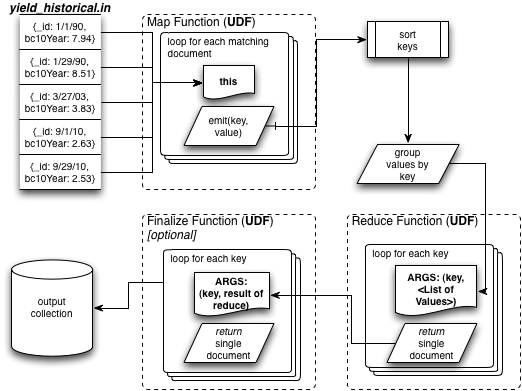
\includegraphics[scale=.42]{images/map_reduce.png}
           \end{center}
           \pagebreak 
           \item The MongoDB JavaScript mapReduce:
           \lstinputlisting{code/mongo_treasury_mr.js}
           \pagebreak
           \item Job Output:
            \lstinputlisting{code/mongo_mr_out.js}
            \pagebreak
            \item A bit more verbosely: 
            \lstinputlisting{code/mongo_mr_out_verbose.js}
            \item Read the collection for your results:
            \lstinputlisting{code/mongo_mr_out_read.js}
            \item It's possible to specify a query, sort and limit as well, to limit your input.
    \end{itemize}
\end{itemizecodeframe}

\subsection{Stored JavaScript Code}
\begin{itemizecodeframe}
    \frametitle{MongoDB's Stored JavaScript}
    \item Each Database has a system collection, `system.js' which can store JavaScript routines
    \item `\_id' is set to the function name, `value' to the function body.
    \item Stored Functions are unique per database and can be accessed in scope from any JavaScript (But not the raw JS Shell)
    \item Useful for commonly used routines in MapReduce
    \item \lstinputlisting{code/stored_func.js}
\end{itemizecodeframe}


\subsection{GeoSpatial Indexes}
\begin{itemizecodeframe}
    \frametitle{GeoSpatial Indexing}
    \item Search by Geospatial proximity with MongoDB\ldots
    \item One Geoindex allowed per database
    \item Index can be created on an array or a subdocument
    \item You must be consistent across all documents (e.g. same key names or order in array)
    \item I loaded the publicly available GTFS data for Caltrain and BART
    \item Quick \& Dirty Python script to create the index:
        \lstinputlisting[language=Python]{code/geospatial_idx.py}
    \item What are the 5 nearest BART or Caltrain stops to our current location (`37.41331, -122.07098')?
        \lstinputlisting[language=JavaScript]{code/geospatial.js}
    \item In production use at Foursquare \& Wordsquared (Formerly Scrabb.ly)
\end{itemizecodeframe}
\subsection{GridFS}

\begin{itemizecodeframe}
    \frametitle{GridFS: Scalable MongoDB File Storage}
    \item Specification for storing large files in MongoDB, supported in all official drivers as reference implementation.
    \item Works around 4MB BSON limit by breaking files into chunks.
    \item Two collections: `fs.files' for metadata, `fs.chunks' stores the individual file chunks.
    \item Sharding: Individual file chunks don't shard but the files themselves will (e.g. File A goes on Server 1, File B goes on Server 2 but no chunks of A will be on 2)
    \item Experimental modules for Lighttpd and Nginx to serve static files directly from GridFS
    \item A Unit Test from Casbah (Scala Driver):
        \lstinputlisting[language=Scala]{code/gridfs_spec.scala}
    \item See the GridFS Spec\ldots \url{http://www.mongodb.org/display/DOCS/GridFS+Specification}
\end{itemizecodeframe}

\subsection{Closing}
\begin{itemizeframe}
    \frametitle{Questions?}
        \item Twitter: {\bf @rit} | mongodb: {\bf @mongodb} | 10gen: {\bf @10gen }
        \item email: {\bf brendan@10gen.com}	
    
    \item Pressing Questions?
    \begin{itemize}
        \item IRC - {freenode.net \bf\#mongodb}
        \item MongoDB Users List - \url{http://groups.google.com/group/mongodb-user}
    \end{itemize}
    \item { 10gen is {\em hiring!}  We need smart engineers in both NY and Bay Area: \url{http://10gen.com/jobs}}
    \item Up Next: ``MongoDB Project Roadmap'' with Dwight Merriman and Eliot Horowitz.  Simulcast to all rooms so stay put!
\end{itemizeframe}


\end{document}
